%last updated in April 2002 by Antje Endemann

\documentclass[runningheads]{llncs}
%In order to omit page numbers and running heads
%please use the following line instead of the first command line:
%\documentclass{llncs}.
%Furthermore change the line \pagestyle{headings} to
%\pagestyle{empty}.
\usepackage{graphicx}
\usepackage{url}
\usepackage{color}
\newcommand {\afbnote} [1] {{\bf \textcolor{red}{(#1)}}}
\newcommand {\ericnote} [1] {{\bf \textcolor{purple}{(#1)}}}
\input{psfig.sty}

\begin{document}

\pagestyle{headings}
%In order to omit page numbers and running heads
%please change this line to
%\pagestyle{empty}
%and change the first command line too, see above.

\mainmatter

\title{Camera pose from face images}

\titlerunning{Camera pose from face images}

\maketitle

\begin{abstract}
\afbnote{todo...}
\end{abstract}

\section{Introduction}
When taking a picture of a human head, the choice of distance from camera to head and focal length (zoom) can have a dramatic effect on the end result.  In Figure \ref{fig:fiducial_migration}, we illustrate the effect of perspective distortion on the face.  The first eight images (in row major order) show a synthetic face (generated using FaceGen \footnote{\url{http://www.facegen.com}}) while varying the distance from camera to head and the focal length.  In the top left image the camera is at a far distance, resulting in a near orthographic projection effect.  The eighth image (bottom row, middle column) the camera is very close to the human head, resulting in an elongated face shape and portruding nose.  Fiducials (corners of eyes/nose/mouth, and nose tip) are marked with red dots.  The bottom right image is the same image as the top left, with fiducial markers from all images.  This illustrates how fiducial features migrate as a function of camera distance and focal length.  In this paper, we show that using imaged 2D fiducial locations are sufficient to recover the distance from camera to head.  Specifically, we show that the distance between camera and any human head can be recovered using a set of exemplar 3D human heads.

\begin{figure}[ht]
\centering
\begin{tabular}{ccc}
\includegraphics[width=.25\linewidth]{resources/figures/extracted_fiducial_0006.png} &
\includegraphics[width=.25\linewidth]{resources/figures/extracted_fiducial_0008.png} &
\includegraphics[width=.25\linewidth]{resources/figures/extracted_fiducial_0001.png} \\
\includegraphics[width=.25\linewidth]{resources/figures/extracted_fiducial_0002.png} &
\includegraphics[width=.25\linewidth]{resources/figures/extracted_fiducial_0003.png} &
\includegraphics[width=.25\linewidth]{resources/figures/extracted_fiducial_0004.png} \\
\includegraphics[width=.25\linewidth]{resources/figures/extracted_fiducial_0005.png} &
\includegraphics[width=.25\linewidth]{resources/figures/extracted_fiducial_0007.png} &
\includegraphics[width=.25\linewidth]{resources/figures/fiducial_migration.png}
\end{tabular}
\caption{A synthetic face at different camera distances and focal length (zoom) to keep the silhouette at a constant size.  Fiducials are shown as red dots.  Bottom left image shows the top left image with fiducials from all camera distances illustrating the migration of fiducials as a function of camera distance/zoom.} 
\label{fig:fiducial_migration}
\end{figure}

\section{Related works}
The specific problem we investigate in this paper is essentially head pose estimation.  Head pose estimation from 2D images is an active field of research, a recent survey can be found in \cite{murphy2009head}.  However, most head pose estimation algorithms focus primarily on the orientation of the head with respect to the camera.  This amounts to estimating the yaw, pitch, and roll egocentric rotation angles of the head.  To our knowledge, existing head pose estimation algorithms do not focus on distance between camera and head (translation in the $z$-axis in figure \ref{fig:head_pose}).

\begin{figure}[ht]
\centering
\includegraphics[width=.7\linewidth]{resources/figures/head_pose.png}
\caption{The goal of head pose estimation is to recover the yaw, pitch, and roll angles of the head, as well as translation along $x$, $y$, and $z$ axes in relation to the camera.  Most head pose estimation algorithms do not test for translation along the $z$-axis.}
\label{fig:head_pose}
\end{figure}

In \cite{liu2003face,liu2006face}, Liu studies the effect of face recognition by humans when viewing faces at different perspective convergence angles (effectively focal length or field of view).  The study involved showing a human test subject images of faces in a training phase, then in a later recognition phase the human subject was shown another image of a face and asked to determine if he had observed this face in the training phase.  The field of view angle was for images in training and recognition phases was changed to see if this had an effect on recognition.  Not surprisingly, their results show that even humans have a hard time recognizing a face when its viewed under different levels of perspective distortion.  This is a motivating factor since if human have trouble with this task, a computer vision algorithm will likely also have the same troubles.  Predicting the distance between camera and face is a first step at mitigating the effects of perspective distortion.

A similar psychology based studied is presented in \cite{perona2007new,bryan2012perspective}.  Here, Perona et al. investigate the effects of perspective distortion as visual cue for social judgement of faces.  Human subjects were asked to judge an image of a face in terms of trustworthiness, attractiveness, and competence.  Their results show that for social judgements, pictures taken from a distance outside of "personal space" (up close) are generally rated lower, while pictures taken at a far distance have higher ratings.

In \cite{ohayon2006robust}, Ohayon and Rivlin present head tracking as a camera pose estimation problem.  Prior to head tracking, 3D points are acquired from the head.  During tracking, correspondences between the 3D points and their imaged 2D points are used to estimate head pose by solving the inverse problem, namely camera pose.  They use the Perspective $n$-Point (PnP) formulation to solve for the camera extrinsic parameters (rotation $R$ and translation $T$).  The PnP method is also known as the Locationi Determination Problem and was first coined in \cite{ransac}.  In effect, the human head is used as a calibration rig.  In this paper, the authors show that head pose can be accurately estimated and tracked under varying yaw/pitch/roll angles and translations about $x$ and $y$ axes.  However, translations about the $z$-axis are not exensively studied.  

\section{Camera pose estimation from face images using EPnP}

Our work is based on \cite{ohayon2006robust}, but we focus primarily on translation along the $z$-axis, which affects the level of induced perspective distortion.  Furthermore, Ohayon and Rivlin present a method for estimating head pose of a specific human head.  We present a method for estimating head pose of human heads in general using a dataset of exemplar human heads. 

\subsection{Efficient Perspective $n$-Point (EP$n$P)}
EPnP is a non-iterative solution to the P$n$P problem.  As stated earlier, the P$n$P problem estimates the pose of a calibrated camera from $n$ 3D-to-2D correspondences.  The advantage of EP$n$P is that the computational complexity grows linearly with $n$, whereas other state-of-the-art methods are $O(n^5)$ or even $O(n^8)$.  We use Matlab code provided by the authors \footnote{\url{http://cvlab.epfl.ch/software/EPnP}}.

\subsection{Exemplar 3D heads}
The geometric configuration of fiducial features does vary from face to face, but in general fiducial locations tend to form clusters, as illustrated in Figure \ref{fig:fiducial_clusters}.  Figure \ref{fig:fiducial_clusters}(a-c) shows point clouds of three different faces taken from the GavaBDB \cite{moreno2004gavabdb} dataset.  Manually clicked fiducial locations are shown in large red dots.  Figure \ref{fig:fiducial_clusters}(c) shows fiducials for 20 different faces, note the fiducials form clusters.  We take advantage of this and use a set of exemplar 3D heads to estimate the camera pose (in particular distance between camera and head) of face images in general. We show that using exemplar heads allows us to accurately estimate the camera pose and distance from camera to the head.

\begin{figure}[h]
\centering
\begin{tabular}{cc}
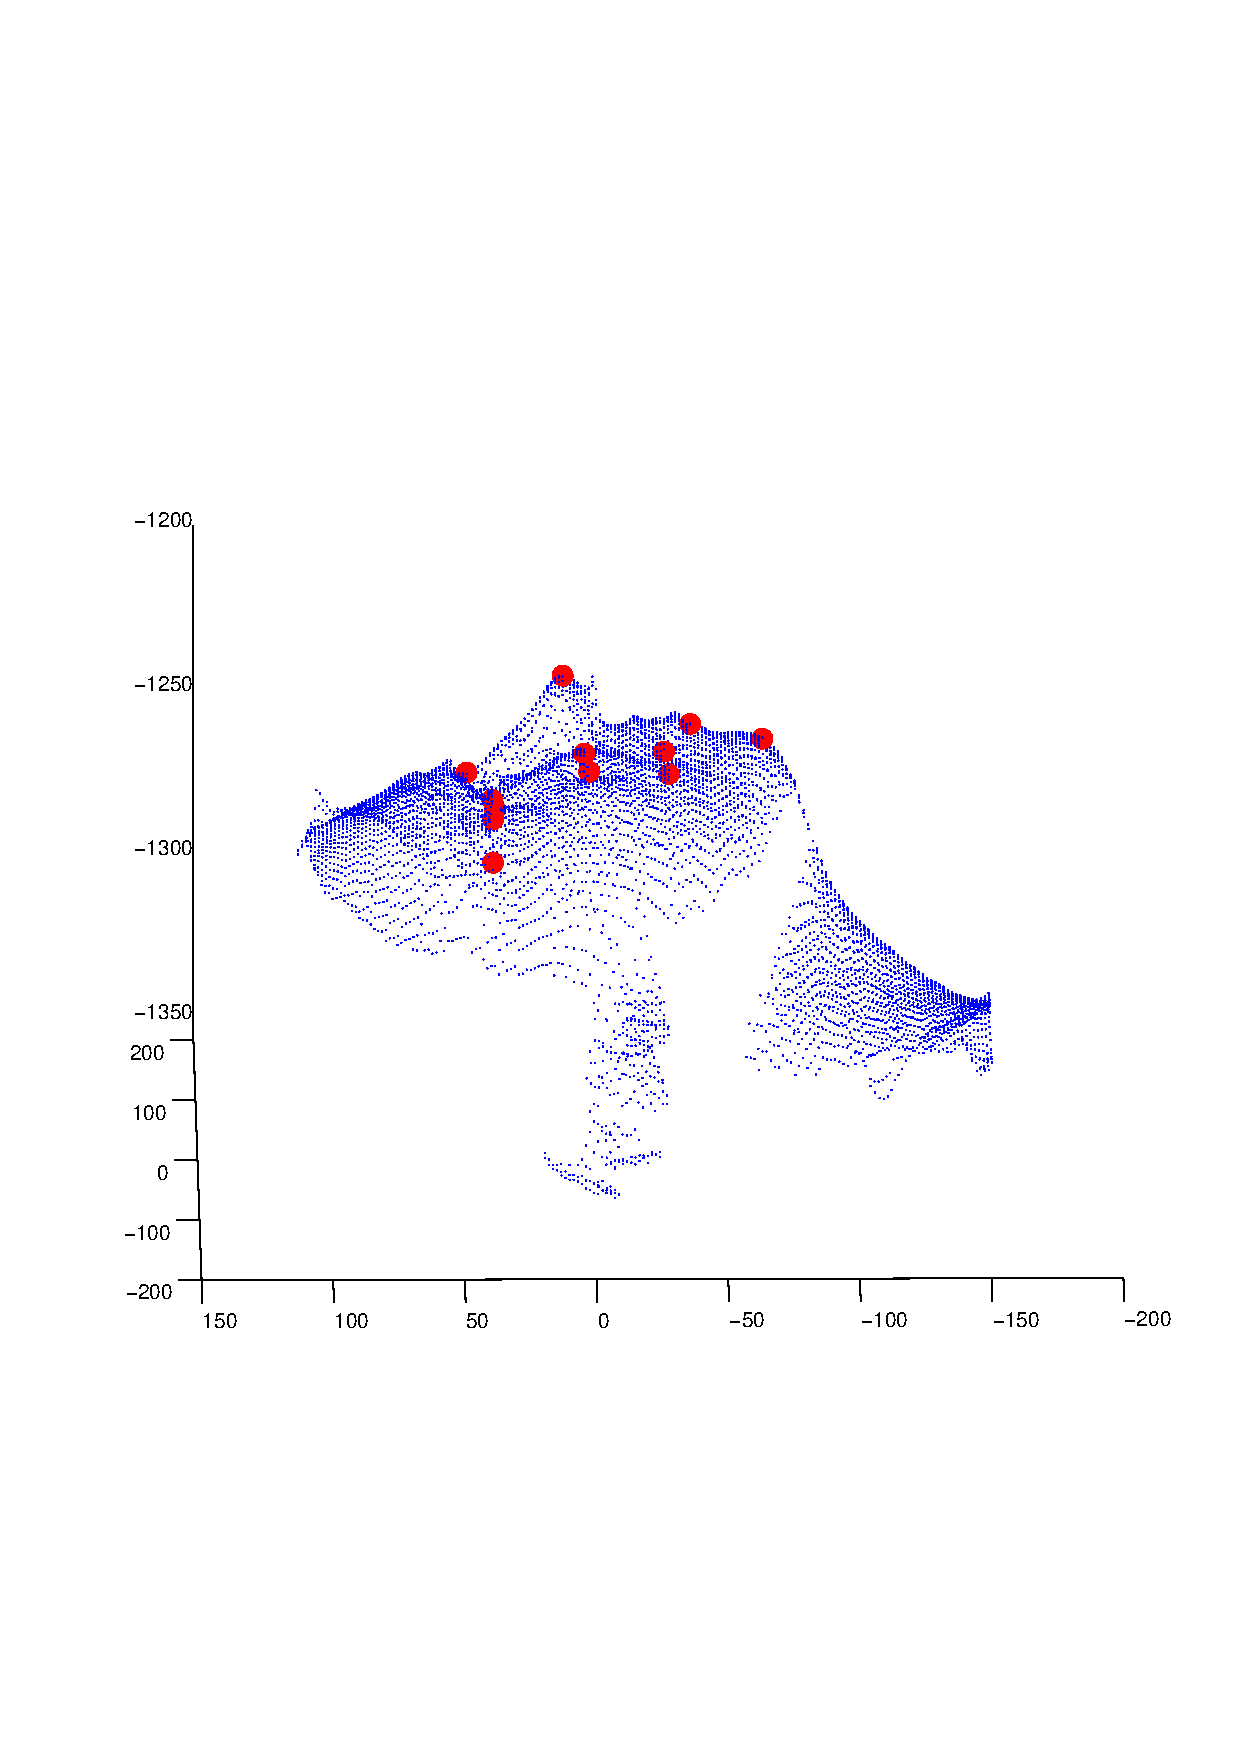
\includegraphics[width=.3\linewidth]{resources/figures/face1.png} &
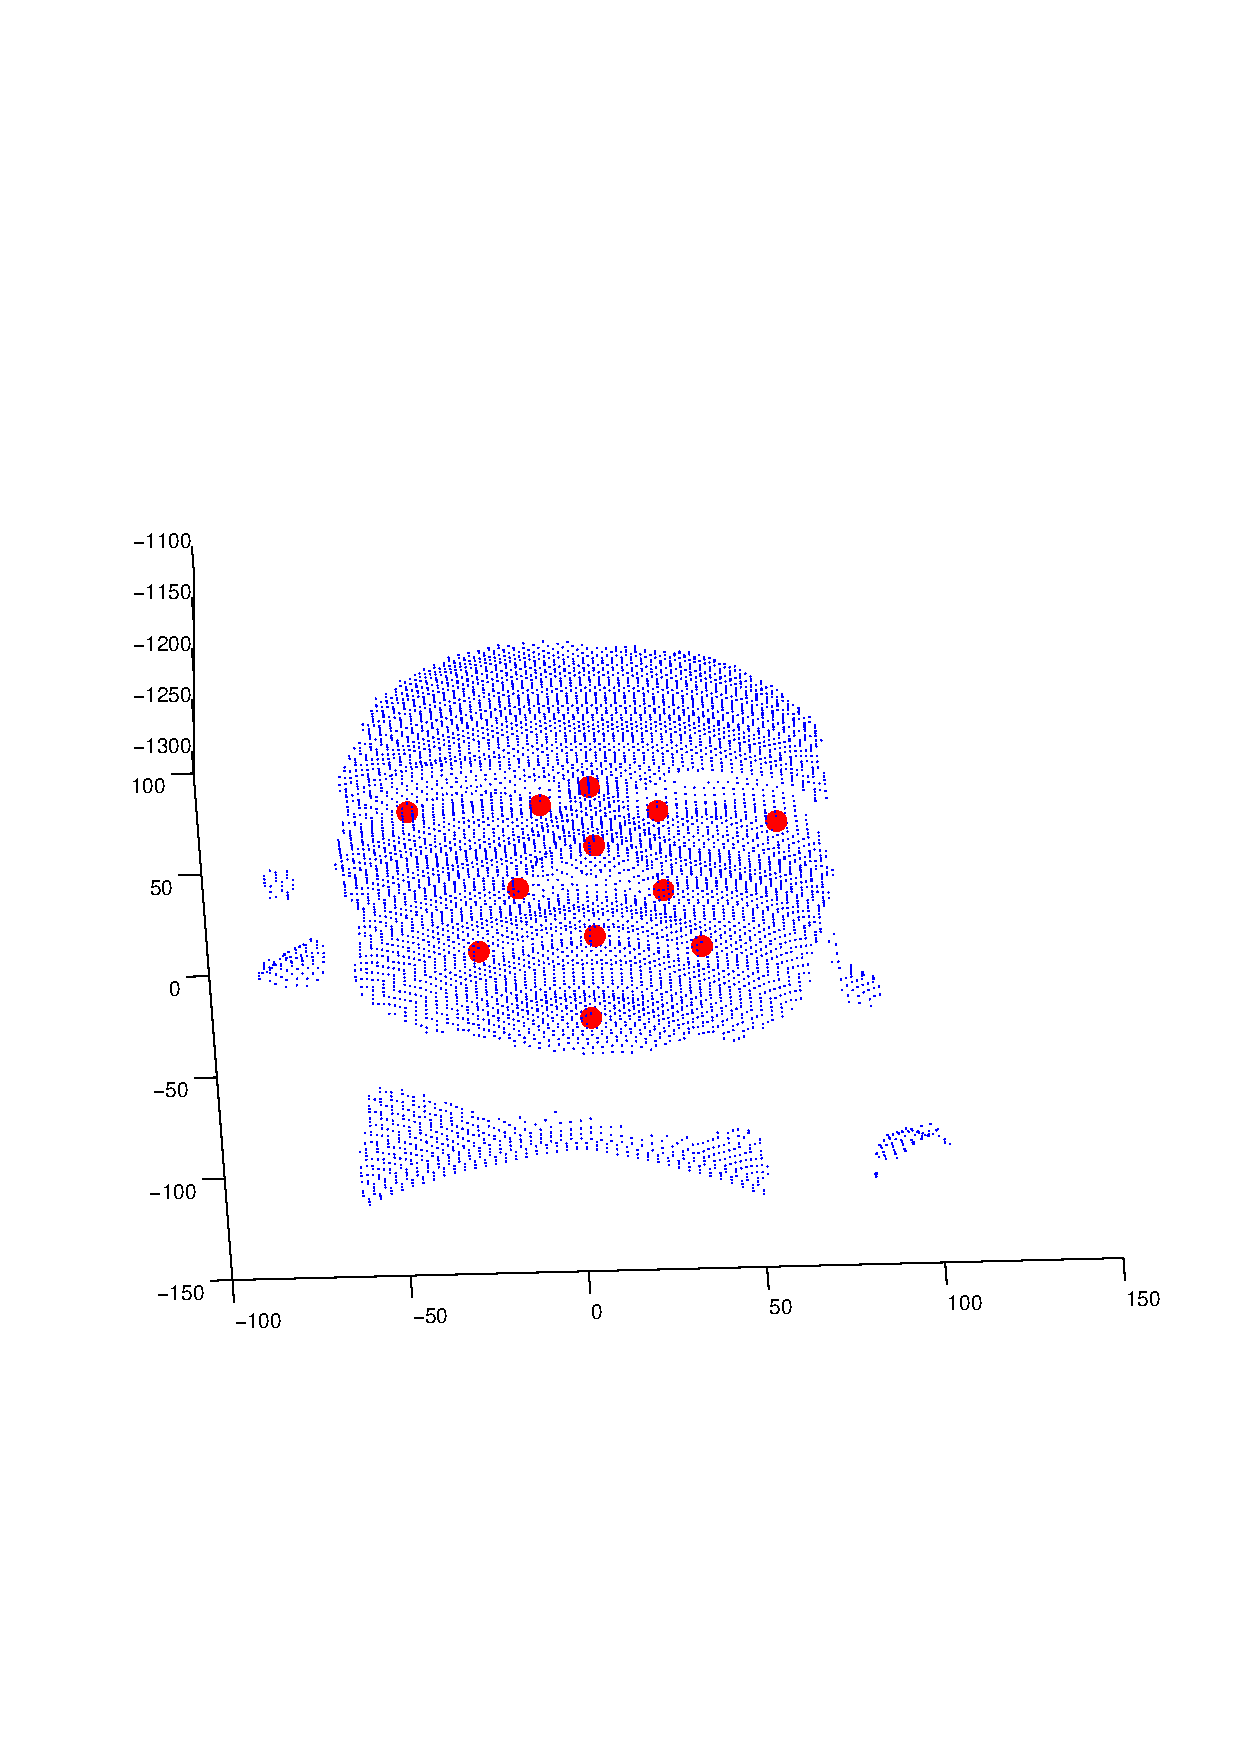
\includegraphics[width=.3\linewidth]{resources/figures/face2.png} \\
(a) & (b) \\
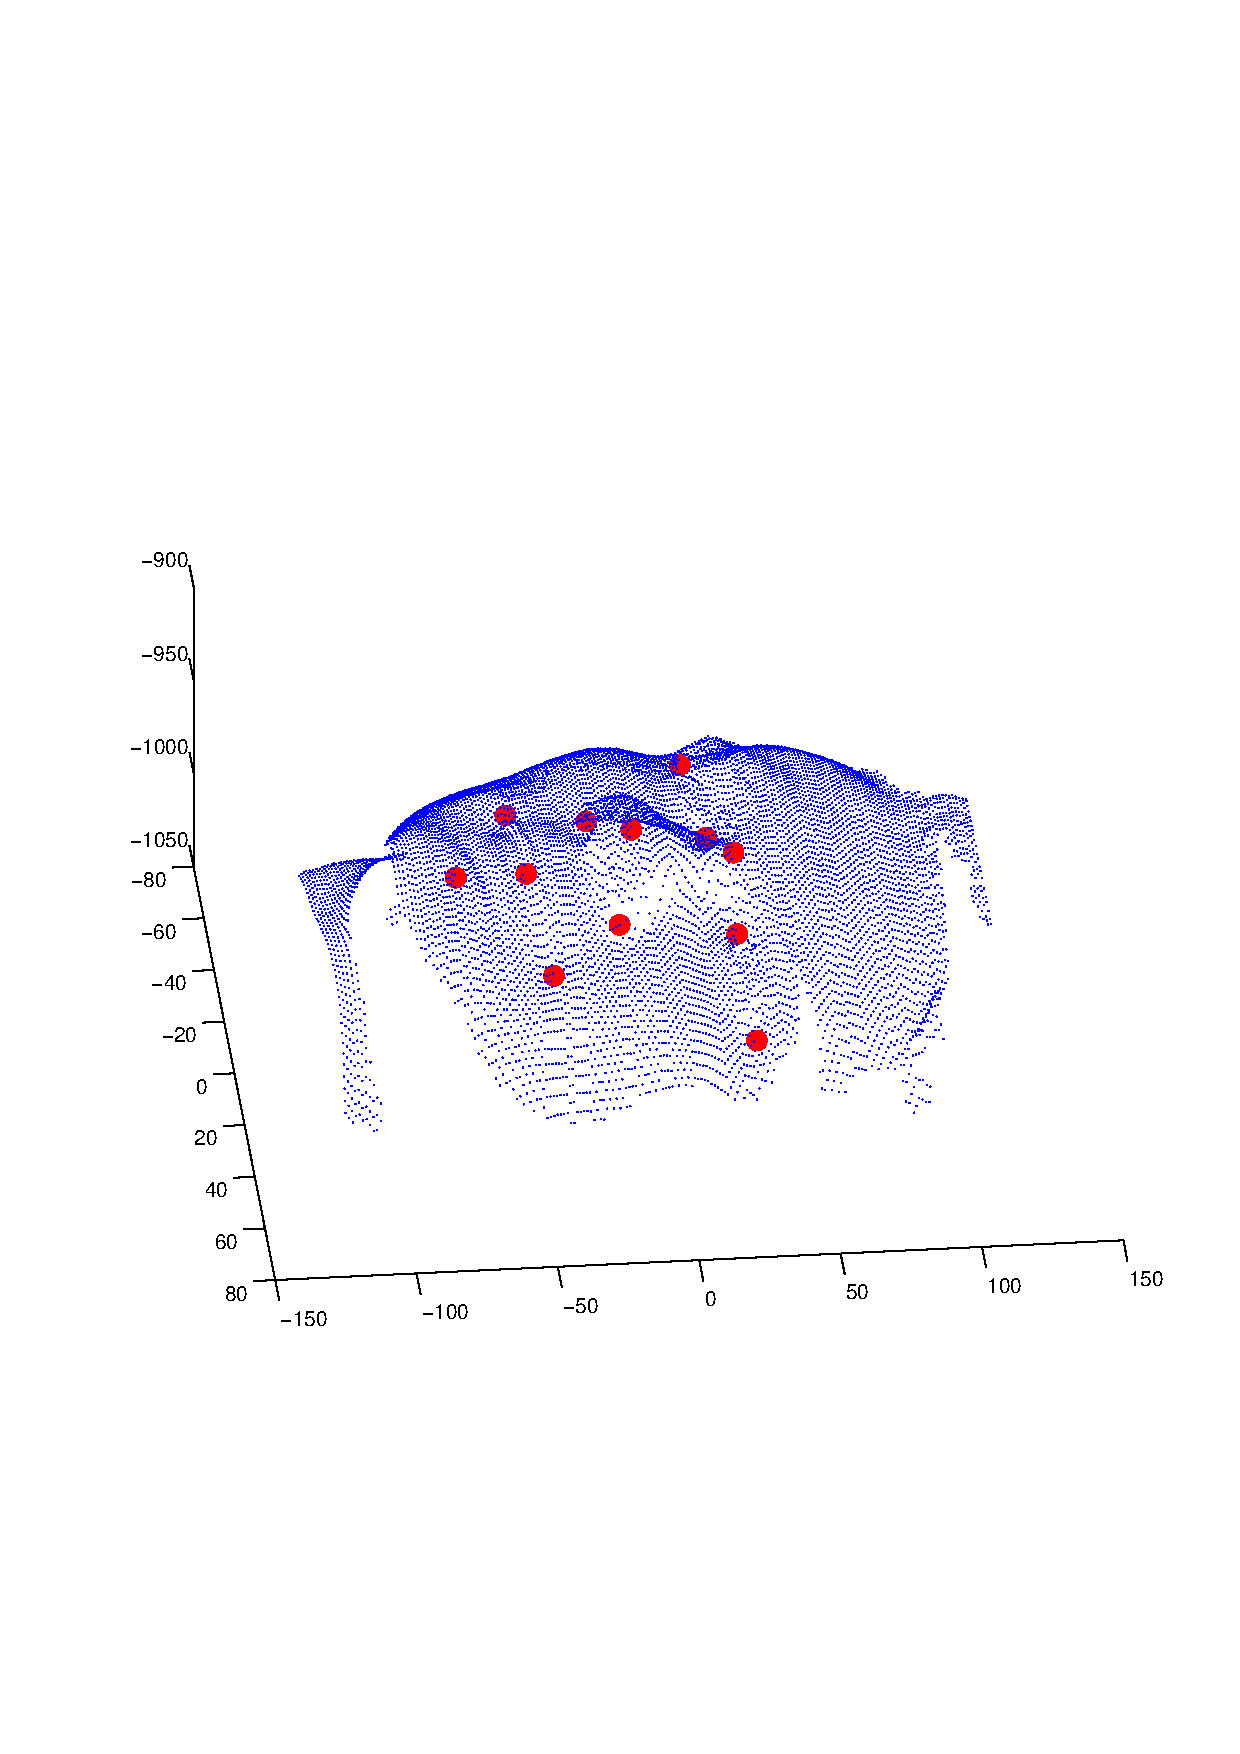
\includegraphics[width=.3\linewidth]{resources/figures/face3.png} &
\includegraphics[width=.5\linewidth]{resources/figures/fiducial_clusters.png} \\
(c) & (d)
\end{tabular}
\caption{(a-b) 3D point clouds of three different faces along with manually clicked fiducials.  (c) Fiducials from 20 faces.}
\label{fig:fiducial_clusters}
\end{figure}

\section{Experimental setup}
In all experiments, we use the Texas 3D Face Recognition Database (Texas 3DFRD) \cite{gupta2010texas}, see figure \ref{fig:t3dfrd}.  This database is a collection of 1149 pairs of frontal facial color and range images of 105 adult human subjects.  Each face also has 25 manually labeled anthropometric facial fiducial points.  Color and range images were captured simultaneously and are thus perfectly registered to each other.  This allows us to have ground truth 3D locations of the fiducial locations.  
\begin{figure}[h]
\centering
\includegraphics[width=.7\linewidth]{resources/figures/t3dfr.jpg}
\caption{Example images from the Texas 3DFRD.}
\label{fig:t3dfrd}
\end{figure}
In this work, we are primarily interested in recovering the distance between camera and head.  Our experiments consist of the following:

\begin{itemize}
\item Project fiducials for a test individual onto an image plane.
\item Use 3D fiducial locations for other individuals as exemplars.
\item For each exemplar, estimate the camera pose (and distance) using EPnP.
\item Final estimate is the average from all exemplars.
\item Repeat while simulating a dolly-zoom camera movement (move camera back, increase focal length).  The focal length is adjusted so as to keep the outermost fiducials close to the eyes at a near constant distance.
\end{itemize}

We perform this experiment for the frontal and $3/4$ profile view of the face.  For the frontal case, we assume all fiducials are visible by the camera.  For the $3/4$ we assume only a subset of the fiducials are visible. In this work, we assume we have a calibrated camera and all intrinsic camera parameters are known.  Simulated camera distances range from approximately 10cm to 100cm

\section{Results}
Figure \ref{fig:results} shows results of camera pose estimation and distance from camera to head.  
\begin{figure}[ht]
\begin{tabular}{cc}
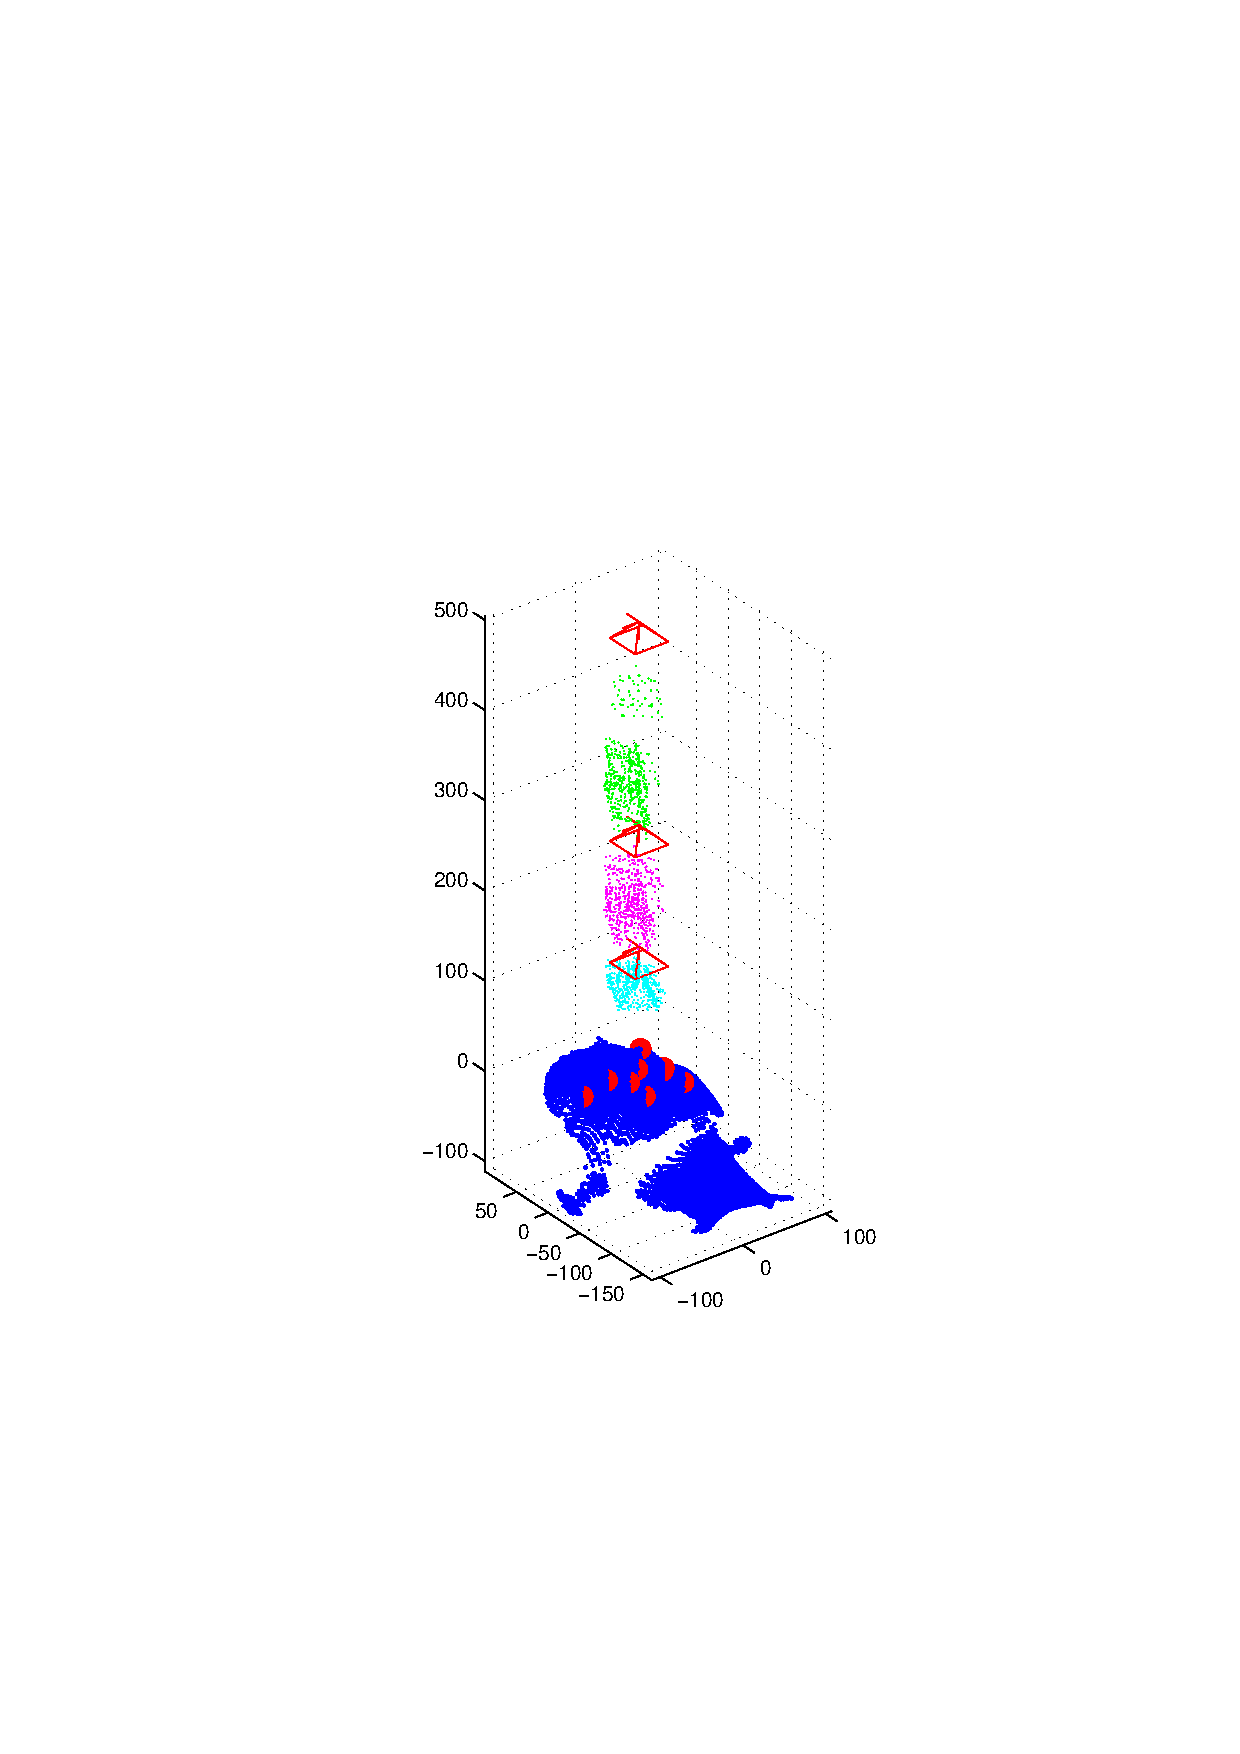
\includegraphics[width=.45\linewidth]{resources/figures/cameraloc_frontal.png} &
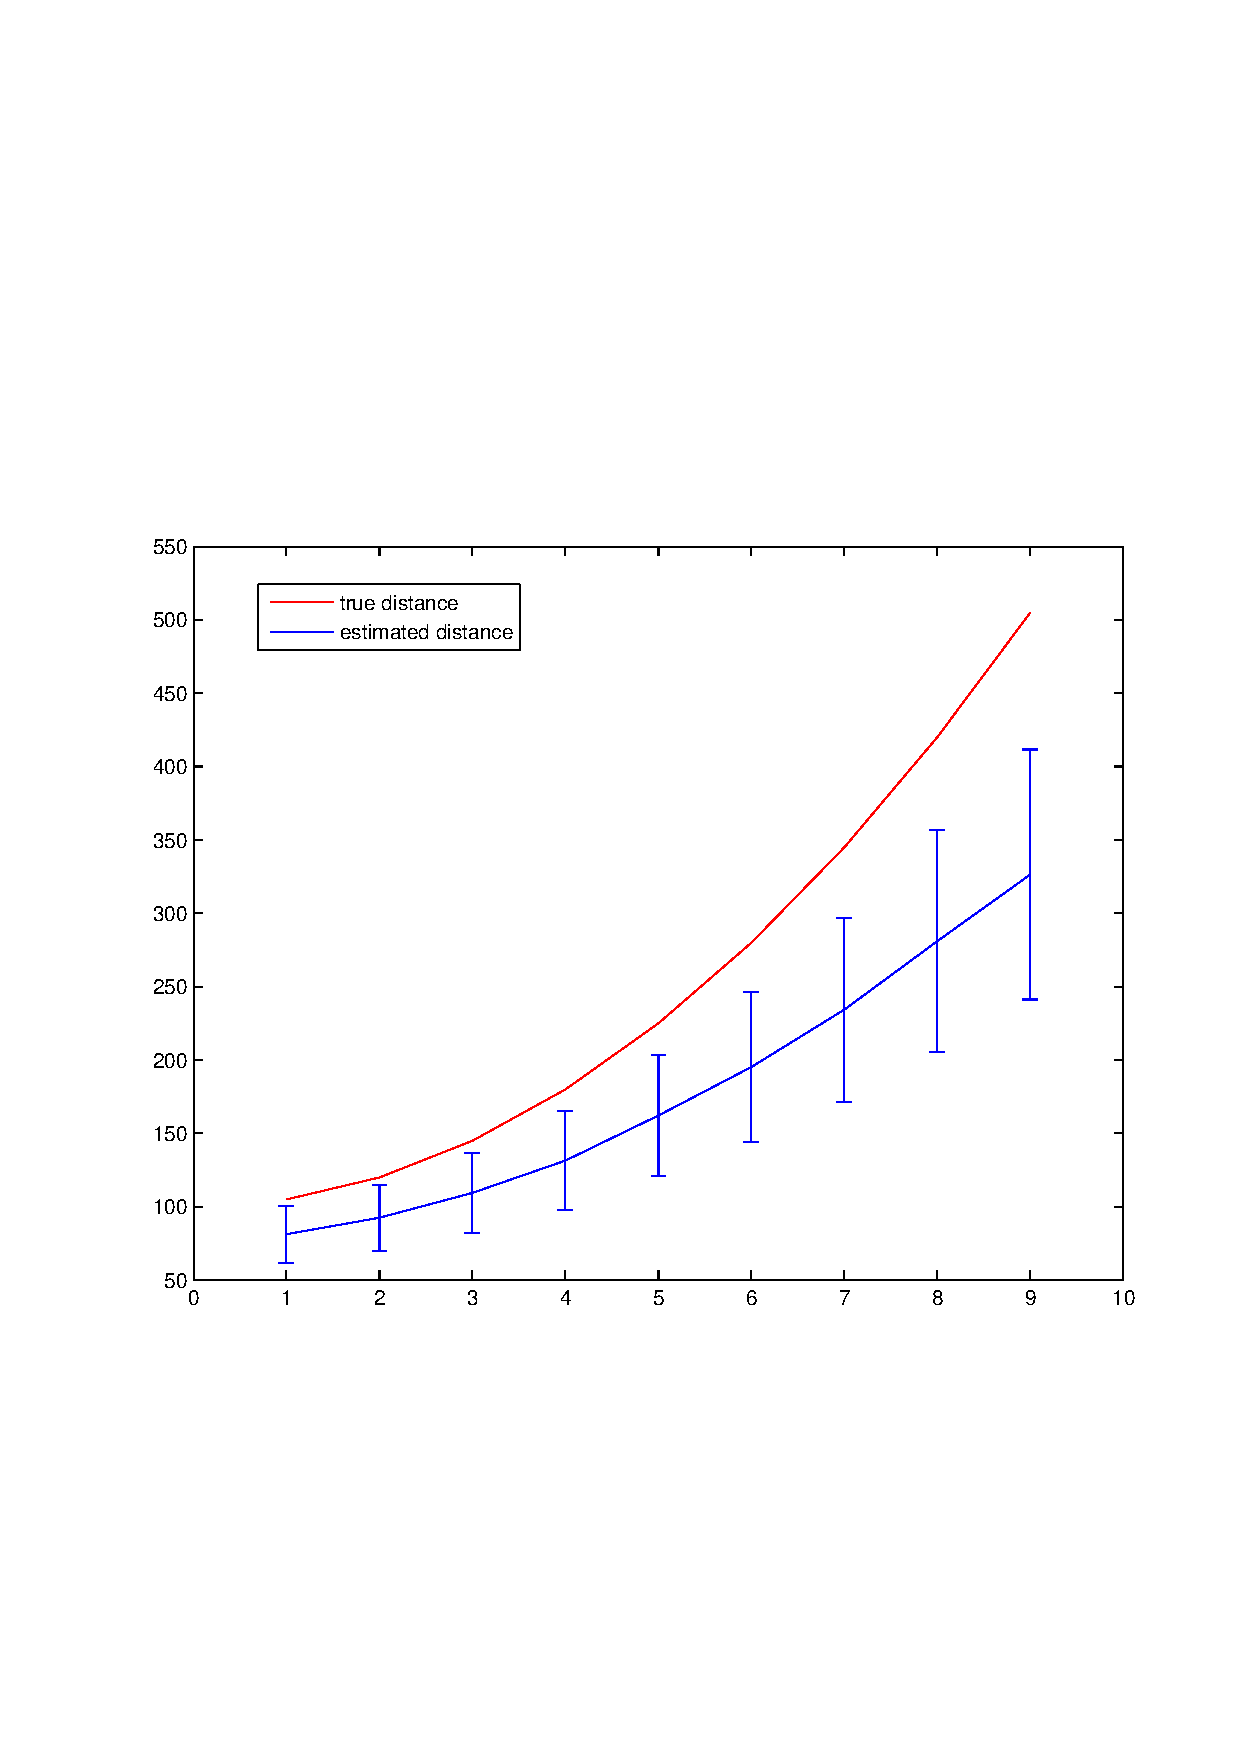
\includegraphics[width=.45\linewidth]{resources/figures/errorbar_frontal.png} \\
(a) & (b) \\
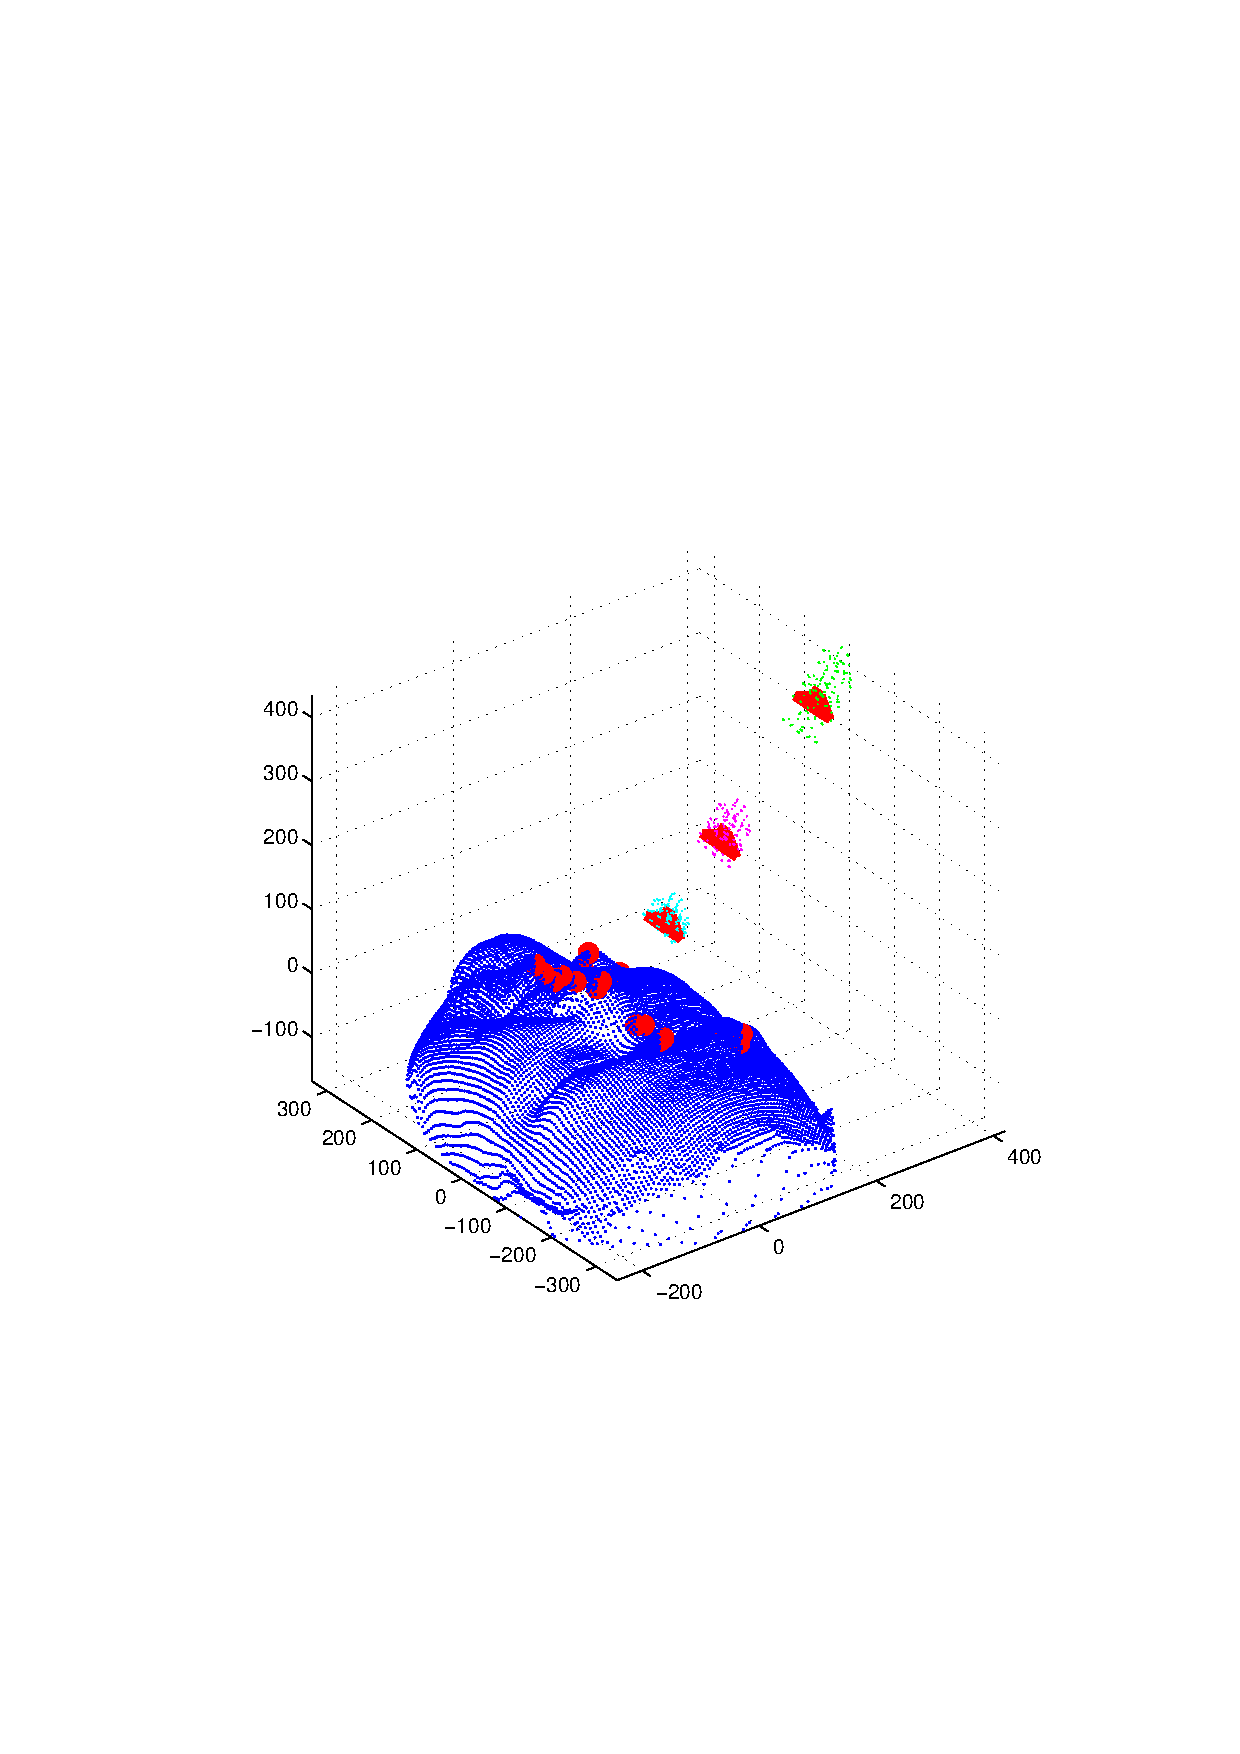
\includegraphics[width=.45\linewidth]{resources/figures/cameraloc_3q.png} &
\includegraphics[width=.45\linewidth]{resources/figures/errorbar_3q.png} \\
(c) & (d)
\end{tabular}
\caption{(a) Camera pose estimation results for the frontal case.  True camera position is the solid red axis.  Estimated camera positions for near/medium/far are shown in cyan/magenta/green respectively.   (b) Distance estimate as an average of exemplar models.  We test nine camera positions and corresponding focal length to keep distance between outermost fiducials next to eye at a near constant. (c) and (d) show similar results for $3/4$ profile view.}
\label{fig:results}
\end{figure}

\afbnote{todo: Show results as a function of number of fiducial points}

\afbnote{todo: Show results for larger simulated distances}

\section{Conclusion}
\afbnote{todo... .  Mention that for this paper we focus on calibrated camera (known intrinsic parameters).  Future work will include uncalibrated case, other methods (appearance based), etc.}

\bibliographystyle{splncs}
\bibliography{library}

\end{document}
